\chapter{Crossfading Sound}

In digital music, it is often useful to crossfade or "mix" between two signals\footnotemark{}. When two signals $A$ and $B$ are used to produce a new signal $C$, crossfading means to control the amount by which signal $C$ is composed of signal $B$ in dependence of the amount by which it is composed of signal $A$. Equation \ref{eq:lcrossfade1} defines the concept of crossfading, in its most basic form, mathematically.

\begin{equation}
  C(t) = (A(t) \cdot x) + (B(t) \cdot (1 - x)), \text{where } x \in [0;1]
  \label{eq:lcrossfade1}
\end{equation}

\footnotetext{Crossfading is most commonly known as the technique a DJ may use to mix between two pieces of music during his/her performance.}

The following sections will examine three techniques of crossfading as described by Daniel R. Mitchell in his book \emph{BasicSynth: Creating a Music Synthesizer in Software}, pages 96 to 99. Additionally, their implementation in C++ will be outlined.

\section{Linear Crossfading}

Linear crossfading is the simplest form of crossfading. Its mathematical definition was already given in Equation \ref{eq:lcrossfade1}, showing that the crossfade value for the "right" signal, $B$, is indirectly proportional to the value for the "left" signal, $A$. This means that when the left value increases, the right value decreases and vice-versa. It should be noted that it is common to provide a range of $[-1;1]$ or $[-100;100]$ (preferred) instead of the mathematically easier range of $[0;1]$, simply to make the interaction more intuitive to the user. Therefore, Equation \ref{eq:lcrossfade1} must be re-formed to Equation \ref{eq:lcrossfade2}. Table \ref{tb:lcrossfade} shows crossfade values alongside the resulting multipliers for signals $A$ and $B$.

\begin{equation}
  C(t) = (A(t) \cdot \frac{100 - x}{200}) + (B(t) \cdot \frac{100 + x}{200}), \text{where } x \in [-100;100]
  \label{eq:lcrossfade2}
\end{equation}

\begin{table}[h!]

  \centering

  \begin{tabular}[]{| l | l | l |}
    \hline
    \rowcolor[gray]{0.8}
    Value & Multiplier $A$ & Multiplier $B$ \\\hline
    -100 & 1 & 0\\\hline
    -75 & 0.875 & 0.125\\\hline
    -50 & 0.75 & 0.25\\\hline
    -25 & 0.625 & 0.375\\\hline
    0 & 0.5 & 0.5\\\hline
    25 & 0.375 & 0.625\\\hline
    50 & 0.25 & 0.75\\\hline
    75 & 0.125 & 0.875\\\hline
    100 & 0 & 1\\
    \hline
  \end{tabular}

  \caption{Crossfade values alongside the resulting multipliers for signals $A$ and $B$.}

  \label{tb:lcrossfade}

\end{table}

\pagebreak

\section{Crossfading with the $\sin$ function}

Another technique of crossfading involves the use of the $\sin$ function to compute the multipliers for signals $A$ and $B$. This is said to improve the "smoothness" of the mix \citebs{98}. Because the $\sin$ function operates with radians, the crossfade values from Equation \ref{eq:lcrossfade2} must be multiplied with $\frac{\pi}{2}$, leading to Equation \ref{eq:scrossfade} for cross-fading with the $\sin$ function. It should be noted that the center value for this technique is not $0.5$, but $\frac{\sqrt{2}}{2}$ or $\sin(\frac{\pi}{4})$. Table \ref{tb:scrossfade} gives cross-fade values using the $\sin$ function and the multipliers that result from them. Figure \ref{fig:lscrossfade} shows how this method of crossfading compares to linear crossfading in a coordinate system.

\begin{equation}
  C(t) = (A(t) \cdot \sin(\frac{100 - x}{200} \cdot \frac{\pi}{2})) + (B(t) \cdot \sin(\frac{100 + x}{200} \cdot \frac{\pi}{2})), \text{where } x \in [-100;100]
  \label{eq:scrossfade}
\end{equation}

\begin{table}[h!]

  \centering

  \begin{tabular}[]{| l | l | l |}
    \hline
    \rowcolor[gray]{0.8}
    Value & Multiplier $A$ & Multiplier $B$ \\\hline
    -100 & 1 & 0\\\hline
    -75 & 0.980 & 0.195\\\hline
    -50 & 0.924 & 0.383\\\hline
    -25 & 0.831 & 0.556\\\hline
    0 & 0.707 & 0.707\\\hline
    25 & 0.556 & 0.831\\\hline
    50 & 0.383 & 0.924\\\hline
    75 & 0.195 & 0.980\\\hline
    100 & 0 & 1\\
    \hline
  \end{tabular}

  \caption{Crossfade values when using the $\sin$ function, alongside the resulting multipliers for signals $A$ and $B$.}

  \label{tb:scrossfade}

\end{table}

\begin{figure}[p!]

  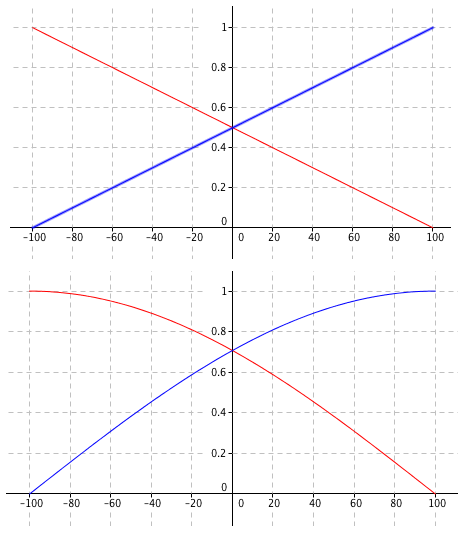
\includegraphics[scale=0.7]{img/lscrossfade}

  \caption{The top graph depicts linear crossfading and the bottom graph crossfading with the $\sin$ function. The red line is the multiplier for signal $A$ and the blue line is the multiplier for signal $B$.}

  \label{fig:lscrossfade}

\end{figure}

\pagebreak

\section{Radical Crossfading}

Another method of non-linear crossfading involves the computation of signal multipliers according to a square-root function. Similar to crossfading with the $\sin$ function, values do not always add up to $1$ for radical crossfading. Moreover, the middle value is again $\frac{\sqrt{2}}{2}$ or $\sin(\frac{\pi}{4})$. Equation \ref{eq:sqrtcrossfade} shows the appropriate mathematical definition for radical crossfading and Table \ref{tb:sqrtcrossfade} displays crossfade values alongside resultant multipliers. Additionally, Figure \ref{fig:sqrtcrossfade} puts radical crossfading into a coordinate-system.

\begin{equation}
  C(t) = (A(t) \cdot \sqrt{\frac{100 - x}{200}}) + (B(t) \cdot \sqrt{\frac{100 + x}{200}}), \text{where } x \in [-100;100]
  \label{eq:sqrtcrossfade}
\end{equation}

\begin{table}[ht!]

  \centering

  \begin{tabular}[]{| l | l | l |}
    \hline
    \rowcolor[gray]{0.8}
    Value & Multiplier $A$ & Multiplier $B$ \\\hline
    -100 & 1 & 0\\\hline
    -75 & 0.935 & 0.354\\\hline
    -50 & 0.866 & 0.500\\\hline
    -25 & 0.791 & 0.612\\\hline
    0 & 0.707 & 0.707\\\hline
    25 & 0.612 & 0.791\\\hline
    50 & 0.500 & 0.866\\\hline
    75 & 0.354 & 0.935\\\hline
    100 & 0 & 1\\
    \hline
  \end{tabular}

  \caption{Radical crossfade values with resultant multipliers for signals $A$ and $B$.}

  \label{tb:sqrtcrossfade}

\end{table}

\begin{figure}[h!]

  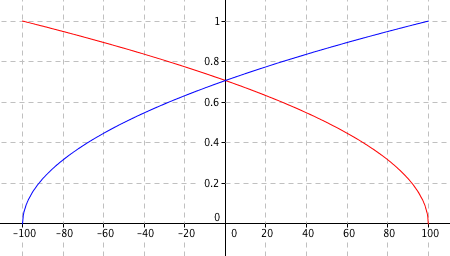
\includegraphics[scale=0.7]{img/sqrtcrossfade}

  \caption{Radical crossfading shown in a coordinate-system. The red line is the multiplier for signal $A$ and the blue line is the multiplier for signal $B$.}

  \label{fig:sqrtcrossfade}

\end{figure}

\pagebreak

\section{Scaling Crossfade values}

It is possible to scale crossfade values resulting from radical crossfading as well as from crossfading with the $\sin$ function in such way that the multipliers at the center crossfade value are again both $0.5$ instead of $\frac{\sqrt{2}}{2}$. To do so, one simply needs to multiply all multipliers by $\frac{\sqrt{2}}{2}$, since $(\frac{\sqrt{2}}{2})^2 = 0.5$. This leads to Equations \ref{eq:scrossfadesc}, for crossfading with the $\sin$ function and \ref{eq:sqrtcrossfadesc} for radical crossfading. Tables \ref{eq:scrossfadesc} and \ref{eq:sqrtcrossfadesc} show the respective multipliers. One natural caveat of scaling is that all values become smaller.

\begin{equation}
  C(t) = (A(t) \cdot \sin(\frac{100 - x}{200} \cdot \frac{\pi}{2}) \cdot \frac{\sqrt{2}}{2}) + (B(t) \cdot \sin(\frac{100 + x}{200} \cdot \frac{\pi}{2}) \cdot \frac{\sqrt{2}}{2}), \text{where } x \in [-100;100]
  \label{eq:scrossfadesc}
\end{equation}

\begin{equation}
  C(t) = (A(t) \cdot \sqrt{\frac{100 - x}{200}} \cdot \frac{\sqrt{2}}{2}) + (B(t) \cdot \sqrt{\frac{100 + x}{200}} \cdot \frac{\sqrt{2}}{2}), \text{where } x \in [-100;100]
  \label{eq:sqrtcrossfadesc}
\end{equation}

\begin{table}[h!]

  \centering

  \begin{tabular}[]{| l | l | l |}
    \hline
    \rowcolor[gray]{0.8}
    Value & Multiplier $A$ & Multiplier $B$ \\\hline
    -100 & 0.707 & 0\\\hline
    -75 & 0.694 & 0.138\\\hline
    -50 & 0.653 & 0.270\\\hline
    -25 & 0.588 & 0.393\\\hline
    0 & 0.5 & 0.5\\\hline
    25 & 0.393 & 0.588\\\hline
    50 & 0.270 & 0.653\\\hline
    75 & 0.138 & 0.694\\\hline
    100 & 0 & 0.707\\
    \hline
  \end{tabular}

  \caption{Scaled values for crossfading with the $\sin$ function, alongside the resulting multipliers for signals $A$ and $B$.}

  \label{tb:scrossfadesc}

\end{table}

\begin{table}[ht!]

  \centering

  \begin{tabular}[]{| l | l | l |}
    \hline
    \rowcolor[gray]{0.8}
    Value & Multiplier $A$ & Multiplier $B$ \\\hline
    -100 & 0.707 & 0\\\hline
    -75 & 0.661 & 0.25\\\hline
    -50 & 0.612 & 0.354\\\hline
    -25 & 0.559 & 0.433\\\hline
    0 & 0.5 & 0.5\\\hline
    25 & 0.433 & 0.559\\\hline
    50 & 0.354 & 0.612\\\hline
    75 & 0.25 & 0.661\\\hline
    100 & 0 & 0.707\\
    \hline
  \end{tabular}

  \caption{Scaled radical crossfade values with resultant multipliers for signals $A$ and $B$.}

  \label{tb:sqrtcrossfade}

\end{table}

\section{Creating Crossfade Tables}

Because crossfade values are constant, i.e. there is only one possible tuple of multipliers for each crossfade value, it was decided that these multipliers should be stored in a table once and then looked-up. This is a lot more efficient than having to calculate each multiplier at every request. Similar to Wavetables, these crossfade tables are stored to a file and then written into computer memory at program start-up. Table \ref{code:crossfadetables} shows a computer program, this time written in the Python programming language, to compute and store crossfade tables.

\begin{table}[hbt!]
  \lstinputlisting[language=Python]{code/crossfadetables.py}
  \caption{}
  \label{code:crossfadetables}
\end{table}
